\subsection{Euler's Method}



\frame{
\begin{block}{}
The reader should be convinced that not all initial value problems can be solved explicitly, and often it is impossible to find a formula for the solution $y(t)$; \\
For example, there is no "closed-form expression" for the solution to $y' = t^3 + y^2$ with $y(0) = 0$. 
\end{block}
\begin{itemize}
\item Hence for engineering and scientific purposes it is necessary to have methods for {\Large approximating the solution}. 
\vspace{0.3cm}
\item If a solution with many significant digits is required, then more computing effort and a sophisticated algorithm must be used. 
\end{itemize}
}

\frame{
The first approach, called {\Large Euler's method}, serves to illustrate the concepts involved in the advanced methods. 
\begin{itemize}
\item It has limited use because of the larger error that is accumulated as the process proceeds. 
\vspace{0.3cm}
\item However, it is important to study because the error analysis is easier to understand. 
\end{itemize}
}

\frame{
\begin{itemize}
\item Let $[a, b]$ be the interval over which we want to find the solution to the well-posed I.V.P. $y' = f(t, y)$ with $y(a) = y_0$. 
\vspace{0.3cm}
\item In actuality, we will not find a differentiable function that satisfies the I.V.P.  
\vspace{0.3cm}
\item Instead, a set of points $\{ ( t_k, y_k)\}$ is generated, and the points are used for an approximation (i.e., $y(t_k) \approx y_k)$.
\end{itemize}
}

\frame{
\begin{center}
How can we proceed to construct {\Large a "set of points"} that will {\Large "satisfy a differential equation approximately"}? 
\end{center}
}

\frame{
\begin{itemize}
\item First we choose the abscissas for the points. 
\item For convenience we subdivide the interval $[a, b]$ into $M$ equal subintervals and select the mesh points 
\begin{equation*}
t_k = a + k h \ \ \ for \ \ \ k = 0,1,\ldots,M \ \ \ where \ h = \frac{b-a}{M}
\end{equation*}
%\begin{figure}
%\begin{center}
%\includegraphics[width=110mm]{fig/ch-6/eq_6-10.png}
%\end{center}
%\end{figure}
\item The value $h$ is called the {\Large step size}. 
\end{itemize}
}

\frame{
We now proceed to solve approximately
\begin{equation}
y' = f(t,y) \ \ over \ \{ t_0 , t_M\}  \ with \ y(t_0) = y_0
\end{equation}
%\begin{figure}
%\begin{center}
%\includegraphics[width=100mm]{fig/ch-6/eq_6-11.png}
%\end{center}
%\end{figure}
Assume that $y(t)$, $y'(t)$, and $y"(t)$ are continuous and use Taylor's theorem to expand $y(t)$ about $t = t_0$.  \\
For each value $t$ there exists a value $C_1$ that lies between $t_0$ and $t$ so that 
\begin{equation*}
y(t) = y(t_0) + y' (t_0)(t - t_0) + \frac{y''(c_1)(t -t_0)^2}{2}
\end{equation*}
%\begin{figure}
%\begin{center}
%\includegraphics[width=100mm]{fig/ch-6/eq_6-12.png}
%\end{center}
%\end{figure}
When $y'(t_0) = f(t_0, y(t_0))$ and $h = h - t_0$ are substituted in equation (6.12), the result is an expression for $y(t_1)$: 
\begin{equation*}
y(t_1) = y(t_0) + h f(t_0,y(t_0)) + y'' (c_1) \frac{h^2}{2}
\end{equation*}
%\begin{figure}
%\begin{center}
%\includegraphics[width=100mm]{fig/ch-6/eq_6-13.png}
%\end{center}
%\end{figure}
}

\frame{
If the step size $h$ is chosen small enough, then we may neglect the second-order term (involving $h^2$) and get 
\begin{equation}
y_1 = y_0 + h f(t_0,y_0),
\end{equation}
%\begin{figure}
%\begin{center}
%\includegraphics[width=80mm]{fig/ch-6/eq_6-14.png}
%\end{center}
%\end{figure}
which is {\Large Euler's approximation}. \\
The process is repeated and generates a sequence of points that approximates the solution curve $y = y(t)$.  \\
The general step for Euler's method is 
\begin{equation*}
t_{k+1} = t_k + h, \ \ \ y_{k+1} = y_k +h f(t_k,y_k) \ \ \ for \  k=0, 1, \ldots, M-1.
\end{equation*}
%\begin{figure}
%\begin{center}
%\includegraphics[width=100mm]{fig/ch-6/eq_6-15.png}
%\end{center}
%\end{figure}
}

\frame{
\begin{block}{Example 6.2.}
Use Euler’s method to solve approximately the initial value problem
\begin{equation}
y′ = Ry \ \ \ over \ [0,1] \ with \ y(0) = y_0 \ and \ R \ constant.
\end{equation}
\end{block}
The step size must be chosen, and then the second formula in (6) can be determined for computing the ordinates.  \\
This formula is sometimes called a difference equation, and in this case it is
\begin{equation}
y_{k+1} =y_k(1+hR) \ \ \ for \ \ k=0, 1, \ldots, M-1.
\end{equation}
}

\frame{
If we trace the solution values recursively, we see that
\begin{equation}
\begin{array}{r l}
y_1 & = y_0(1+hR) \\
y_2 & = y_1(1+hR) = y_0(1+hR)2 \\
& \vdots \\
y_M & = yM-1(1+hR)=y_0 (1+hR)^M.
\end{array}
\end{equation}
%\begin{figure}
%\begin{center}
%\includegraphics[width=110mm]{fig/ch-6/ex_6-2.png}
%\end{center}
%\end{figure}
%\begin{figure}
%\begin{center}
%\includegraphics[width=110mm]{fig/ch-6/ex_6-2_2.png}
%\end{center}
%\end{figure}
}

\frame{
For most problems there is no explicit formula for determining the solution points, 
and each new point must be computed successively from the previous point. \\
However, for the initial value problem (7) we are fortunate; 
Euler’s method has the explicit solution
\begin{equation}
t_k = kh \ \ \ \ y_k = y_0 ( 1 + h R )^k \ \ \ for \ \  k=0, 1, \ldots, M.
\end{equation}
Formula (10) can be viewed as the “compound interest” formula, and the Euler approximation gives the future value of a deposit.
}

\frame{
\begin{block}{Example 9.3.}
Suppose that $\$1000$ is deposited and earns $10\%$ interest compounded continuously over 5 years. 
What is the value at the end of $5$ years?
\end{block}
We choose to use Euler approximations with $h = 1$, $\frac{1}{12}$ , and $\frac{1}{360}$ to approximate $y(5)$ for the I.V.P. :
\begin{equation}
y' = 0.1 y \ \ \ over \ \ [0,5] \ \ with \ \ y(0) = 1000
\end{equation}
the above formula  with $R = 0.1$ produces the following table \footnote{Table 6.1}.
%\begin{figure}
%\begin{center}
%\includegraphics[width=110mm]{fig/ch-6/ex_6-3.png}
%\end{center}
%\end{figure}
\begin{figure}
\begin{center}
%\includegraphics[width=60mm]{fig/ch-6/tab_6-1.png}
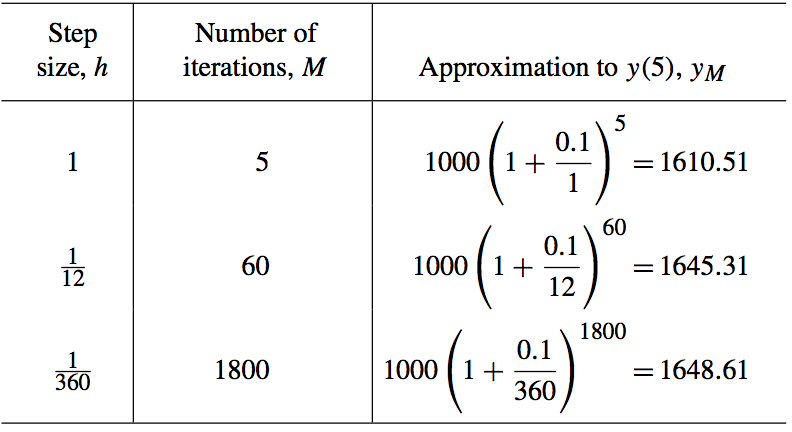
\includegraphics[width=60mm]{chap-6/tab_9-1.png}
\end{center}
\end{figure}
}





\frame{
\begin{itemize}
\item Think about the different values $y_5$, $y_{60}$, and $y_{I800}$ that are used to determine the future value after $5$ years. 
\item These values are obtained using different step sizes and reflect different amounts of computing effort to obtain an approximation to $y(5)$. 
\item The solution to the I.V.P. is $y(5) = 1000e^{0.5} = 1648.72$. 
\item If we did not use the closed-form solution (6.19), then it would have required $1800$ iterations of Euler's method to obtain $y_{1800}$, and we still have only five digits of accuracy in the answer!
\end{itemize}
}

\frame{
\begin{itemize}
\item If bankers had to approximate the solution to the I.V.P. (6.16), they would choose Euler's method because of the explicit formula in (6.19). 
\item The more sophisticated methods for approximating solutions do not have an explicit formula for finding $y_k$, but they will require less computing effort. 
\end{itemize}
}

\frame{
\frametitle{Geometric Description}
\begin{itemize}
\item If you start at the point $(t_0, y_0)$ and compute the value of the slope $m_0 = f(t_0, y_0)$ and move horizontally the amount $h$ and vertically $hf(t_0, y_0)$, then you are moving along the tangent line to $y(t)$ and will end up at the point $(t_1, y_1)$ (see Figure 6.5). 
\item Notice that $(t_1, y_1)$ is not on the desired solution curve! 
%\item But this is the approximation that we are generating. 
\item Hence we must use $(t_1, y_1)$ as though it were correct and proceed by computing the slope $m_1 = f(t_1, y_1)$ and using it to obtain the next vertical displacement $hf(t_1, y_1)$ to locate $(t_2, y_2)$, and so on. 
\end{itemize}
\begin{figure}
\begin{center}
%\includegraphics[width=60mm]{fig/ch-6/fig_6-5.png}
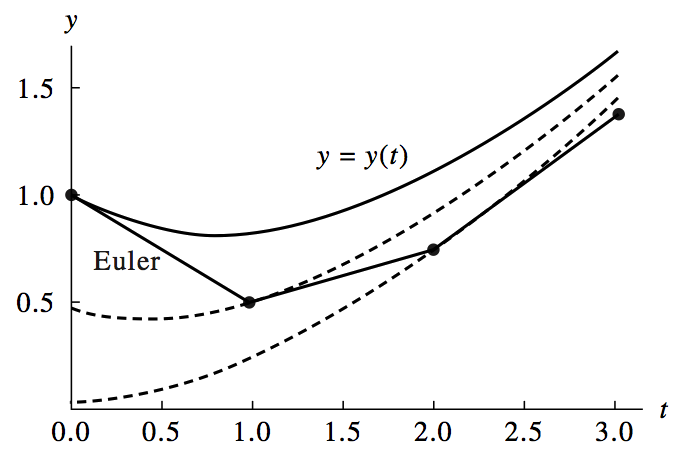
\includegraphics[width=45mm]{chap-6/fig_9-5.png}
\end{center}
\end{figure}
}

\frame{
\frametitle{Step Size versus Error}
\begin{itemize}
\item The methods we introduce for approximating the solution of an initial value problem are called {\Large difference methods} or {\Large discrete variable methods}. 
\item The solution is approximated at a set of discrete points called a grid (or mesh) of points. 
\item An elementary single-step method has the form $y_{k+1} = y_k + h \Phi (t_k, y_k)$ for some function $\Phi$ called an {\Large increment junction}. 
\end{itemize}
When using any discrete variable method to solve an initial value problem approximately, there are two sources of error: discretization and round off. 
}

\frame{
\begin{block}{Definition 6.3.}
Assume that $\{ (t_k, y_k)\}_{k=0}^M$ is the set of discrete approximations and that $y = y(t)$ is the unique solution to the initial value problem. 
\begin{itemize}
\item The {\Large global discretization error} $e_k$ is defined by 
\begin{equation}
e_k =y(t_k)-y_k \ \ \ for \ \ \  k=0, 1, \ldots, M.
\end{equation}
%\begin{figure}
%\begin{center}
%\includegraphics[width=90mm]{fig/ch-6/eq_6-20.png}
%\end{center}
%\end{figure}
It is the difference between the unique solution and the solution obtained by the discrete variable method. 
\item The {\Large local discretization error} $e_{k+1}$ is defined by 
\begin{equation}
e_{k+1} = y(t_{k+1})-y_k -h\Phi(t_k,y_k) \ \ \ for \ \ k=0, 1, \ldots, M-1.
\end{equation}
%\begin{figure}
%\begin{center}
%\includegraphics[width=90mm]{fig/ch-6/eq_6-21.png}
%\end{center}
%\end{figure}
It is the error committed in the single step from $t_k$ to $t_{k+1}$· 
\end{itemize}
\end{block}
}

\frame{
\begin{itemize}
\item When we obtained equation (6.15) for Euler's method, the neglected term for each step was $y^{(2)}(c_k)(h^2/2)$. 
\item If this was the only error at each step, then at the end of the interval $[a, b]$, after $M$ steps have been made, the accumulated error would be 
\begin{equation}
\sum_{k=1}^M y^{(2)}(c_k) \frac{h^2}{2} \approx M_y^{(2)} (c) \frac{h^2}{2} = \frac{hM}{2}y^{(2)}(c) h 
= \frac{(b-a)y^{(2)}(c)}{2} h = O(h^1)
\end{equation}
%\begin{figure}
%\begin{center}
%\includegraphics[width=90mm]{fig/ch-6/p_255.png}
%\end{center}
%\end{figure}
\item There could be more error, but this estimate predominates. 
\item A detailed discussion on this topic can be found in advanced texts on numerical methods for differential equations. 
\end{itemize}
}

\frame{
\begin{block}{Theorem 6.3 (Precision of Euler’s Method).}
Assume that $y(t)$ is the solution to the I.V.P. given in (2). 
If $y(t) \in C^2 [t_0, b]$ and $\{(t_k, y_k)\}^M_{k=0}$ is the sequence of approximations generated by Euler’s method, 
then
\begin{equation}
\begin{array}{l l}
|e_k| & = |y(t_k) - y_k| = O(h), \\ 
& \\
|e_{k+1}| & = |y(t_{k+1}) - y_k - hf(t_k,y_k)| = O(h^2).
\end{array}
\end{equation}
The error at the end of the interval is called the {\Large final global error (F.G.E.)} :
\begin{equation}
E(y(b), h) = |y(b) - y_M| = O(h).
\end{equation}
\end{block}
%\begin{figure}
%\begin{center}
%\includegraphics[width=110mm]{fig/ch-6/theorem_6-3.png}
%\end{center}
%\end{figure}
}

\frame{
\begin{block}{Remark.}
\begin{itemize}
\item The final global error $E(y(b), h)$ is used to study the behavior of the error for various step sizes. 
\vspace{0.5cm}
\item It can be used to give us an idea of how much computing effort must be done to obtain an accurate approximation. 
\end{itemize}
\end{block}
}

\frame{
Examples 6.4 and 6.5 illustrate the concepts in Theorem 6.3. 
If approximations are computed using the step sizes $h$ and $h/2$, we should have 
\begin{equation}
E (y(b), h) \approx C_h
\end{equation}
%\begin{figure}
%\begin{center}
%\includegraphics[width=80mm]{fig/ch-6/eq_6-24.png}
%\end{center}
%\end{figure}
for the larger step size, and
\begin{equation}
E \left( y(b), \frac{h}{2} \right) \approx C \frac{h}{2} = \frac{1}{2} Ch \approx \frac{1}{2} E(y(b),h)
\end{equation}
%\begin{figure}
%\begin{center}
%\includegraphics[width=90mm]{fig/ch-6/eq_6-25.png}
%\end{center}
%\end{figure}
Hence the idea in Theorem 6.3 is that if the step size in Euler's method is reduced by a factor of $\frac{1}{2}$, we can expect that the overall F.G.E. will be reduced by a factor of $\frac{1}{2}$. 
}

\frame{
\begin{block}{Example 6.4.}
Use Euler’s method to solve the I.V.P.
\begin{equation}
y' = \frac{t-y}{2} \ \ \ on \ \ [0,3] \ \ with \ \ y(0) = 1 
\end{equation}
\end{block}

\begin{figure}
\begin{center}
%\includegraphics[width=90mm]{fig/ch-6/fig_6-6.png}
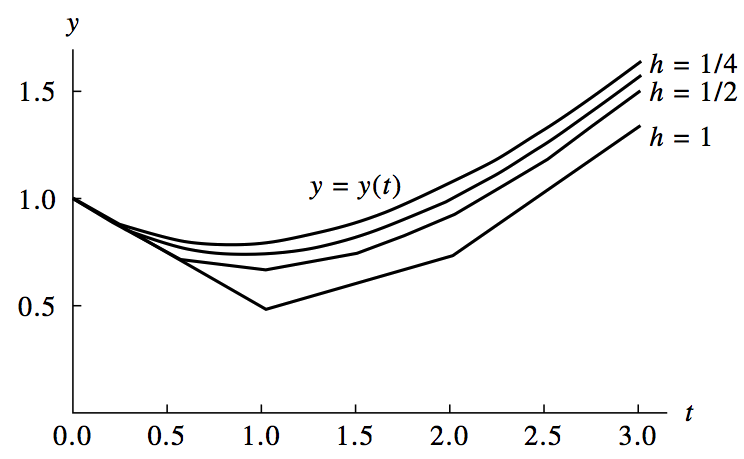
\includegraphics[width=60mm]{chap-6/fig_9-6.png}
\end{center}
\end{figure}
Figure 6.6 shows graphs of the four Euler solutions and the exact solution curve $y(t) = 3e^{-t \slash 2} - 2 + t$. \\
}

\frame{
Table 6.2 gives the values for the four solutions at selected abscissas. 
\begin{figure}
\begin{center}
%\includegraphics[width=80mm]{fig/ch-6/tab_6-2.png}
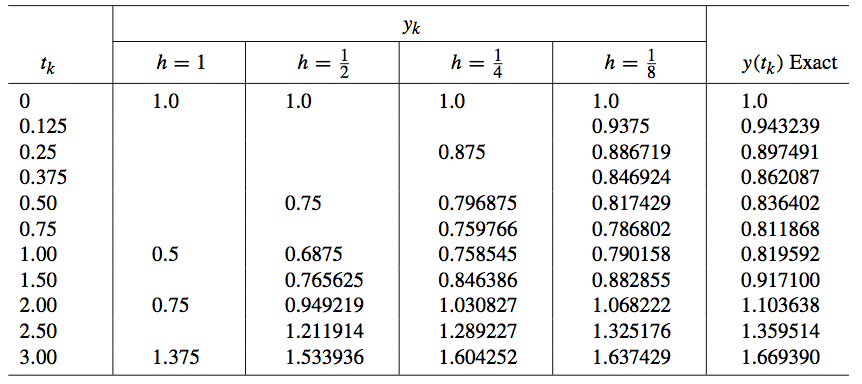
\includegraphics[width=80mm]{chap-6/tab_9-2.png}
\end{center}
\end{figure}

For the step size $h = 0.25$, the calculations are
\begin{equation}
\begin{array}{r l}
y_1 & = 1.0+0.25 \left( \frac{0.0-1.0}{2} \right) = 0.875 \\
& \\
y_2 & =  0.875 + 0.25 \left( \frac{0.25-0.875}{2} \right) = 0.796875, \hspace{0.3cm}	etc.
\end{array}
\end{equation}
%\begin{figure}
%\begin{center}
%\includegraphics[width=110mm]{fig/ch-6/ex_6-4.png}
%\end{center}
%\end{figure}
%\begin{figure}
%\begin{center}
%\includegraphics[width=90mm]{fig/ch-6/p_256.png}
%\end{center}
%\end{figure}
This iteration continues until we arrive at the last step: 
\begin{equation}
y(3) \approx y_{12} = 1.440573 + 0.25\left( \frac{2.75 - 1.440573 }{2} \right) = 1.604252
\end{equation}
%\begin{figure}
%\begin{center}
%\includegraphics[width=90mm]{fig/ch-6/p_256_2.png}
%\end{center}
%\end{figure}
}

%\frame{
%
%}

\frame{
\begin{block}{Example 6.5.}
Compare the F.G.E. when Euler’s method is used to solve the I.V.P.
\begin{equation}
y^{(1)} = \frac{t-y}{2} \ \ \ over \ \ \  [0,3] \ \ \ with \ \ y(0) = 1,
\end{equation}
using step sizes $1$, $\frac{1}{2}$, $\ldots$, $\frac{1}{64}$
\end{block}
%\begin{figure}
%\begin{center}
%\includegraphics[width=110mm]{fig/ch-6/ex_6-5.png}
%\end{center}
%\end{figure}
%Table 6.3 gives the F.G.E. for several step sizes and shows that the error in the approximation to $y(3)$ decreases by about $\frac{1}{2}$ when the step size is reduced by a factor of $\frac{1}{2}$. 
For the smaller step sizes the conclusion of Theorem 6.3 is easy to see: 
\begin{equation}
E(y(3),h)=y(3)-y_M = O(h') \approx C_h, \ \ \ where   C=0.256.
\end{equation}
%\begin{figure}
%\begin{center}
%\includegraphics[width=100mm]{fig/ch-6/p_257.png}
%\end{center}
%\end{figure}
\begin{figure}
\begin{center}
%\includegraphics[width=80mm]{fig/ch-6/tab_6-3.png}
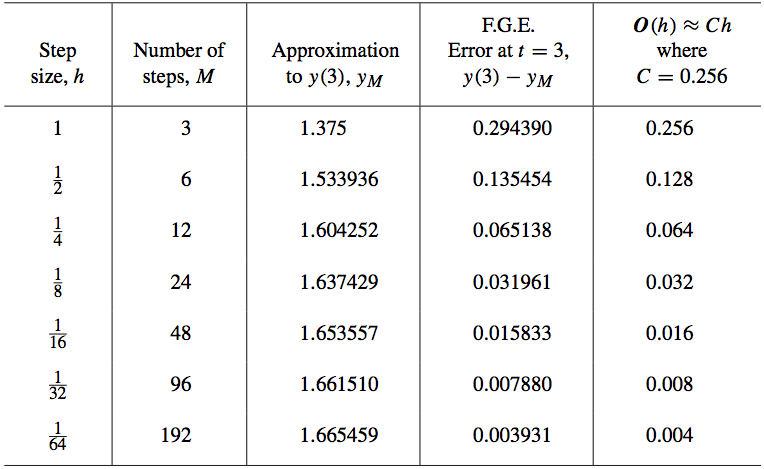
\includegraphics[width=55mm]{chap-6/tab_9-3.png}
\end{center}
\end{figure}
}

%\frame{
%\begin{figure}
%\begin{center}
%\includegraphics[width=110mm]{fig/ch-6/prog_6-1.png}
%\end{center}
%\end{figure}
%}

